\documentclass{article}
%\usepackage{fullpage}
%\usepackage{nopageno} 
\usepackage[margin=1.5in]{geometry}
\usepackage{tikz}
\usetikzlibrary{shapes.geometric, calc}
\usepackage{amsmath}
\usepackage{amssymb}
\usepackage[normalem]{ulem}
\usepackage{fancyhdr}
\usepackage{cancel}
\usepackage{enumerate}
%\renewcommand\headheight{12pt}
\pagestyle{fancy}
\lhead{May 2, 2014}
\rhead{Jon Allen}
\allowdisplaybreaks

\newcommand{\abs}[1]{\left\lvert #1 \right\rvert}

\begin{document}
Part 2 (3 points): Due in class Friday, May 2.

Chapter 8: \#33 (just the first part where you calculate R7 and R8), and the problems below.

Schroder exercise 1: Draw the dissection of the 11-gon that corresponds to the bracketing ( a1 ( ( a2 a3 a4 a5 ) a6 ) (a7 (a8 a9) a10 ) ).

Schroder exercise 2: Draw the Schroder paths from (0,0) to (6,0). Verify that exactly half have no horizontal steps on the x-axis.
\section*{Chapter 8}
\begin{enumerate}
\setcounter{enumi}{31}
  \item
  Use the recurrence relation (8.31) to compute the small Schr\"{o}der numbers $s_8$ and $s_9$.

  We are given the $s_1$ through $s_7$ on page 310. They are $1,1,3,11,45,197,903,\dots$
  \begin{align*}
    0&=(n+2)s_{n+2}-3(2n+1)s_{n+1}+(n-1)s_n\\
    s_{n+2}&=\frac{3(2n+1)}{n+2}s_{n+1}+\frac{1-n}{n+2}s_n\\
    s_{n}&=\frac{3(2(n-2)+1)}{(n-2)+2}s_{n-1}+\frac{1-(n-2)}{(n-2)+2}s_{n-2}\\
    s_{n}&=\frac{3(2n-3)}{n}s_{n-1}+\frac{3-n}{n}s_{n-2}\\
    s_8&=\frac{3\cdot13}{8}\cdot903-\frac{5}{8}\cdot197\\
    &=4279\\
    s_9&=\frac{3\cdot15}{9}\cdot4279-\frac{6}{9}\cdot903\\
    &=20793
  \end{align*}

  \item
  (just the first part where you calculate R7 and R8)

  Use the recurrence relation (8.32) to compute the large Schr\"{o}der numbers $R_7$ and $R_8$. Verify that $R_7=2s_8$ and $R_8=2s_9$, as stated in Corollary 8.5.8.
\begin{align*}
  R_n&=R_{n-1}+\sum\limits_{k=0}^{n-1}{R_kR_{n-1-k}},\quad(n\ge1)\\
  R_0&=1\\
  R_1&=1+1=2\\
  R_2&=2+2+2=6\\
  R_3&=6+6+4+6=22\\
  R_4&=22+22+12+12+22=90\\
  R_5&=90+90+44+36+44+90=270+88+36=394\\
  R_6&=394+394+180+132+132+180+394=1806\\
  R_7&=1806+1806+788+540+484+540+788+1806=8558\\
  R_8&=8558+8558+3612+2364+1980+1980+2364+3612+8558=41586\\
\end{align*}
And since I accidentally did \#32 anyhow, I could as well do the second part. $41586/2=20793$ and $8558/2=4279$
\end{enumerate}
\section*{Schr\"{o}der Exercises}
\begin{enumerate}
  \item
  Draw the dissection of the 11-gon that corresponds to the bracketing $( a_1 ( ( a_2 a_3 a_4 a_5 ) a_6 ) (a_7 (a_8 a_9) a_{10} ) )$.
  
  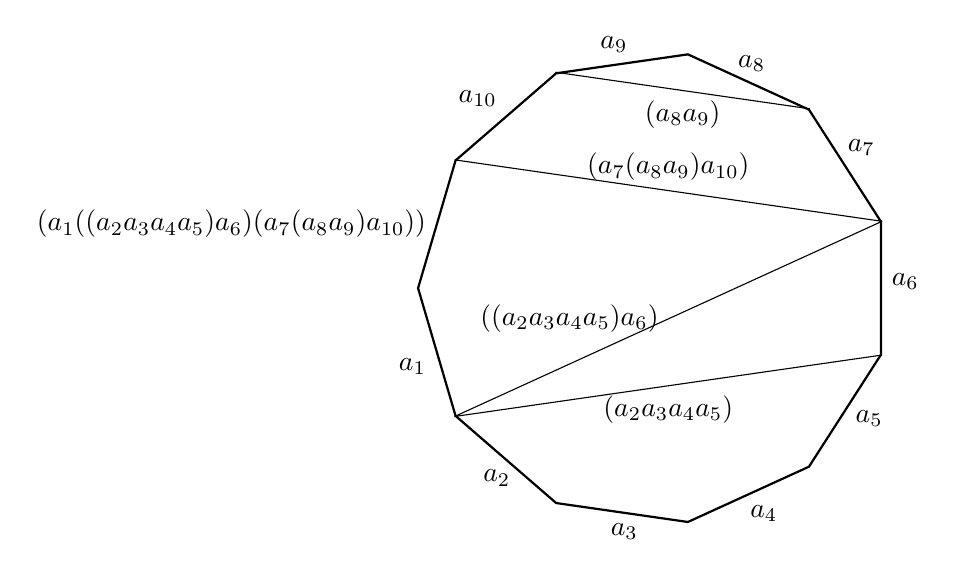
\begin{tikzpicture}
    \node (pol) [draw, thick, black,rotate=90,minimum size=6cm,regular polygon, regular polygon sides=11] at (0,0) {}; 

    \foreach \n [count=\nu from 1, remember=\n as \lastn, evaluate={\nu+\lastn}] in {1,2,...,10} 
    \node[anchor=\n*(360/11)]at(pol.side \n){$a_{\nu}$};
    \draw (pol.corner 8) -- node[anchor=north]{$(a_8 a_9)$}(pol.corner 10);
    \draw (pol.corner 7) -- node[anchor=south]{$(a_7(a_8 a_9)a_{10})$}(pol.corner 11);
    \draw (pol.corner 2) -- node[anchor=north]{$(a_2a_3a_4a_5)$}(pol.corner 6);
    \draw (pol.corner 2) -- node[anchor=east]{$((a_2a_3a_4a_5)a_6)$}(pol.corner 7);
    \node[anchor=360]at(pol.side 11){$(a_1((a_2a_3a_4a_5)a_6)(a_7(a_8 a_9)a_{10}))$};
  \end{tikzpicture}

  \item
  Draw the Schroder paths from $(0,0)$ to $(6,0)$. Verify that exactly half have no horizontal steps on the $x$-axis.

  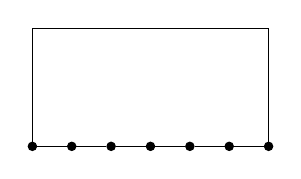
\begin{tikzpicture}[every node/.style={draw,shape=circle,fill=black,inner sep=0pt,minimum size=3pt}]
  \path (0,0) node (p0) {} (.5,0) node (p1) {} (1,0) node (p2) {}
  (1.5,0) node (p3) {} (2,0) node (p4) {} (2.5,0) node (p5) {} (3,0) node (p6) { };
  \draw (p0) -- (p1) -- (p2) -- (p3) -- (p4) -- (p5) -- (p6);
  \draw (0,0) -- (0,1.5) -- (3,1.5) -- (3,0);
  \end{tikzpicture}
  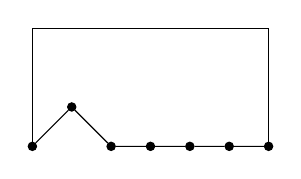
\begin{tikzpicture}[every node/.style={draw,shape=circle,fill=black,inner sep=0pt,minimum size=3pt}]
  \path (0,0) node (p0) {} (.5,.5) node (p1) {} (1,0) node (p2) {}
  (1.5,0) node (p3) {} (2,0) node (p4) {} (2.5,0) node (p5) {} (3,0) node (p6) { };
  \draw (p0) -- (p1) -- (p2) -- (p3) -- (p4) -- (p5) -- (p6);
  \draw (0,0) -- (0,1.5) -- (3,1.5) -- (3,0);
  \end{tikzpicture}
  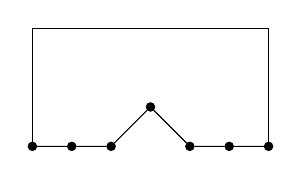
\begin{tikzpicture}[every node/.style={draw,shape=circle,fill=black,inner sep=0pt,minimum size=3pt}]
  \path (0,0) node (p0) {} (.5,0) node (p1) {} (1,0) node (p2) {}
  (1.5,.5) node (p3) {} (2,0) node (p4) {} (2.5,0) node (p5) {} (3,0) node (p6) { };
  \draw (p0) -- (p1) -- (p2) -- (p3) -- (p4) -- (p5) -- (p6);
  \draw (0,0) -- (0,1.5) -- (3,1.5) -- (3,0);
  \end{tikzpicture}
  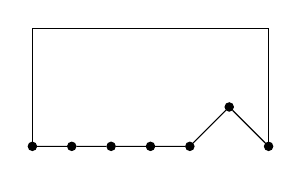
\begin{tikzpicture}[every node/.style={draw,shape=circle,fill=black,inner sep=0pt,minimum size=3pt}]
  \path (0,0) node (p0) {} (.5,0) node (p1) {} (1,0) node (p2) {}
  (1.5,0) node (p3) {} (2,0) node (p4) {} (2.5,.5) node (p5) {} (3,0) node (p6) { };
  \draw (p0) -- (p1) -- (p2) -- (p3) -- (p4) -- (p5) -- (p6);
  \draw (0,0) -- (0,1.5) -- (3,1.5) -- (3,0);
  \end{tikzpicture}
  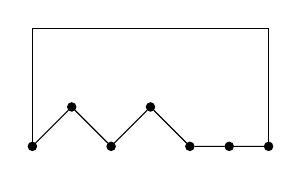
\begin{tikzpicture}[every node/.style={draw,shape=circle,fill=black,inner sep=0pt,minimum size=3pt}]
  \path (0,0) node (p0) {} (.5,.5) node (p1) {} (1,0) node (p2) {}
  (1.5,.5) node (p3) {} (2,0) node (p4) {} (2.5,0) node (p5) {} (3,0) node (p6) { };
  \draw (p0) -- (p1) -- (p2) -- (p3) -- (p4) -- (p5) -- (p6);
  \draw (0,0) -- (0,1.5) -- (3,1.5) -- (3,0);
  \end{tikzpicture}
  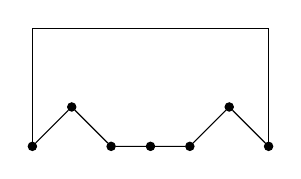
\begin{tikzpicture}[every node/.style={draw,shape=circle,fill=black,inner sep=0pt,minimum size=3pt}]
  \path (0,0) node (p0) {} (.5,.5) node (p1) {} (1,0) node (p2) {}
  (1.5,0) node (p3) {} (2,0) node (p4) {} (2.5,.5) node (p5) {} (3,0) node (p6) { };
  \draw (p0) -- (p1) -- (p2) -- (p3) -- (p4) -- (p5) -- (p6);
  \draw (0,0) -- (0,1.5) -- (3,1.5) -- (3,0);
  \end{tikzpicture}
  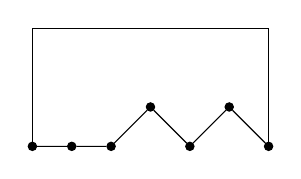
\begin{tikzpicture}[every node/.style={draw,shape=circle,fill=black,inner sep=0pt,minimum size=3pt}]
  \path (0,0) node (p0) {} (.5,0) node (p1) {} (1,0) node (p2) {}
  (1.5,.5) node (p3) {} (2,0) node (p4) {} (2.5,.5) node (p5) {} (3,0) node (p6) { };
  \draw (p0) -- (p1) -- (p2) -- (p3) -- (p4) -- (p5) -- (p6);
  \draw (0,0) -- (0,1.5) -- (3,1.5) -- (3,0);
  \end{tikzpicture}
  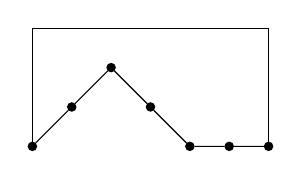
\begin{tikzpicture}[every node/.style={draw,shape=circle,fill=black,inner sep=0pt,minimum size=3pt}]
  \path (0,0) node (p0) {} (.5,.5) node (p1) {} (1,1) node (p2) {}
  (1.5,.5) node (p3) {} (2,0) node (p4) {} (2.5,0) node (p5) {} (3,0) node (p6) { };
  \draw (p0) -- (p1) -- (p2) -- (p3) -- (p4) -- (p5) -- (p6);
  \draw (0,0) -- (0,1.5) -- (3,1.5) -- (3,0);
  \end{tikzpicture}
  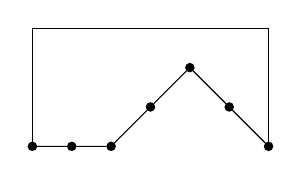
\begin{tikzpicture}[every node/.style={draw,shape=circle,fill=black,inner sep=0pt,minimum size=3pt}]
  \path (0,0) node (p0) {} (.5,0) node (p1) {} (1,0) node (p2) {}
  (1.5,.5) node (p3) {} (2,1) node (p4) {} (2.5,.5) node (p5) {} (3,0) node (p6) { };
  \draw (p0) -- (p1) -- (p2) -- (p3) -- (p4) -- (p5) -- (p6);
  \draw (0,0) -- (0,1.5) -- (3,1.5) -- (3,0);
  \end{tikzpicture}
  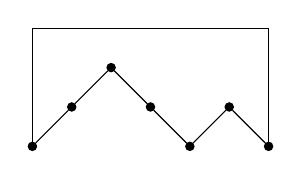
\begin{tikzpicture}[every node/.style={draw,shape=circle,fill=black,inner sep=0pt,minimum size=3pt}]
  \path (0,0) node (p0) {} (.5,.5) node (p1) {} (1,1) node (p2) {}
  (1.5,.5) node (p3) {} (2,0) node (p4) {} (2.5,.5) node (p5) {} (3,0) node (p6) { };
  \draw (p0) -- (p1) -- (p2) -- (p3) -- (p4) -- (p5) -- (p6);
  \draw (0,0) -- (0,1.5) -- (3,1.5) -- (3,0);
  \end{tikzpicture}
  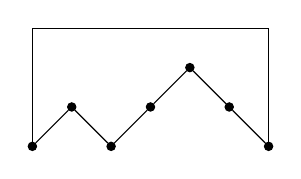
\begin{tikzpicture}[every node/.style={draw,shape=circle,fill=black,inner sep=0pt,minimum size=3pt}]
  \path (0,0) node (p0) {} (.5,.5) node (p1) {} (1,0) node (p2) {}
  (1.5,.5) node (p3) {} (2,1) node (p4) {} (2.5,.5) node (p5) {} (3,0) node (p6) { };
  \draw (p0) -- (p1) -- (p2) -- (p3) -- (p4) -- (p5) -- (p6);
  \draw (0,0) -- (0,1.5) -- (3,1.5) -- (3,0);
  \end{tikzpicture}
  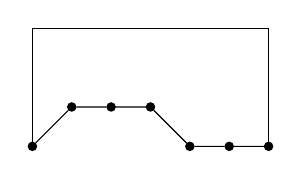
\begin{tikzpicture}[every node/.style={draw,shape=circle,fill=black,inner sep=0pt,minimum size=3pt}]
  \path (0,0) node (p0) {} (.5,.5) node (p1) {} (1,.5) node (p2) {}
  (1.5,.5) node (p3) {} (2,0) node (p4) {} (2.5,0) node (p5) {} (3,0) node (p6) { };
  \draw (p0) -- (p1) -- (p2) -- (p3) -- (p4) -- (p5) -- (p6);
  \draw (0,0) -- (0,1.5) -- (3,1.5) -- (3,0);
  \end{tikzpicture}
  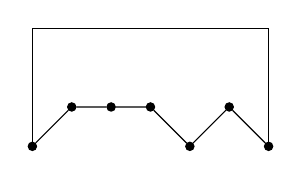
\begin{tikzpicture}[every node/.style={draw,shape=circle,fill=black,inner sep=0pt,minimum size=3pt}]
  \path (0,0) node (p0) {} (.5,.5) node (p1) {} (1,.5) node (p2) {}
  (1.5,.5) node (p3) {} (2,0) node (p4) {} (2.5,.5) node (p5) {} (3,0) node (p6) { };
  \draw (p0) -- (p1) -- (p2) -- (p3) -- (p4) -- (p5) -- (p6);
  \draw (0,0) -- (0,1.5) -- (3,1.5) -- (3,0);
  \end{tikzpicture}
  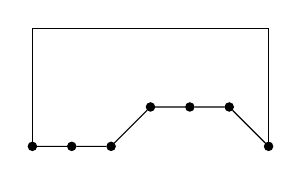
\begin{tikzpicture}[every node/.style={draw,shape=circle,fill=black,inner sep=0pt,minimum size=3pt}]
  \path (0,0) node (p0) {} (.5,0) node (p1) {} (1,0) node (p2) {}
  (1.5,.5) node (p3) {} (2,.5) node (p4) {} (2.5,.5) node (p5) {} (3,0) node (p6) { };
  \draw (p0) -- (p1) -- (p2) -- (p3) -- (p4) -- (p5) -- (p6);
  \draw (0,0) -- (0,1.5) -- (3,1.5) -- (3,0);
  \end{tikzpicture}
  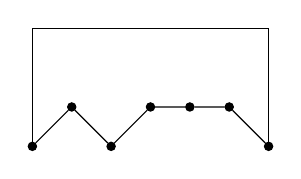
\begin{tikzpicture}[every node/.style={draw,shape=circle,fill=black,inner sep=0pt,minimum size=3pt}]
  \path (0,0) node (p0) {} (.5,.5) node (p1) {} (1,0) node (p2) {}
  (1.5,.5) node (p3) {} (2,.5) node (p4) {} (2.5,.5) node (p5) {} (3,0) node (p6) { };
  \draw (p0) -- (p1) -- (p2) -- (p3) -- (p4) -- (p5) -- (p6);
  \draw (0,0) -- (0,1.5) -- (3,1.5) -- (3,0);
  \end{tikzpicture}
  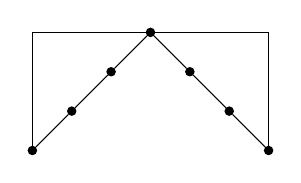
\begin{tikzpicture}[every node/.style={draw,shape=circle,fill=black,inner sep=0pt,minimum size=3pt}]
  \path (0,0) node (p0) {} (.5,.5) node (p1) {} (1,1) node (p2) {}
  (1.5,1.5) node (p3) {} (2,1) node (p4) {} (2.5,.5) node (p5) {} (3,0) node (p6) { };
  \draw (p0) -- (p1) -- (p2) -- (p3) -- (p4) -- (p5) -- (p6);
  \draw (0,0) -- (0,1.5) -- (3,1.5) -- (3,0);
  \end{tikzpicture}
  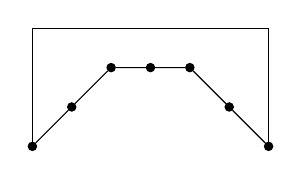
\begin{tikzpicture}[every node/.style={draw,shape=circle,fill=black,inner sep=0pt,minimum size=3pt}]
  \path (0,0) node (p0) {} (.5,.5) node (p1) {} (1,1) node (p2) {}
  (1.5,1) node (p3) {} (2,1) node (p4) {} (2.5,.5) node (p5) {} (3,0) node (p6) { };
  \draw (p0) -- (p1) -- (p2) -- (p3) -- (p4) -- (p5) -- (p6);
  \draw (0,0) -- (0,1.5) -- (3,1.5) -- (3,0);
  \end{tikzpicture}
  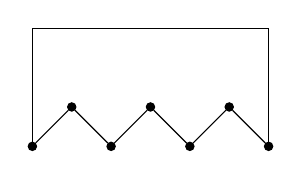
\begin{tikzpicture}[every node/.style={draw,shape=circle,fill=black,inner sep=0pt,minimum size=3pt}]
  \path (0,0) node (p0) {} (.5,.5) node (p1) {} (1,0) node (p2) {}
  (1.5,.5) node (p3) {} (2,0) node (p4) {} (2.5,.5) node (p5) {} (3,0) node (p6) { };
  \draw (p0) -- (p1) -- (p2) -- (p3) -- (p4) -- (p5) -- (p6);
  \draw (0,0) -- (0,1.5) -- (3,1.5) -- (3,0);
  \end{tikzpicture}
  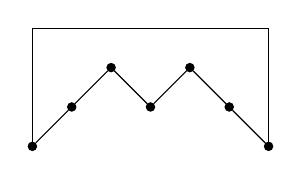
\begin{tikzpicture}[every node/.style={draw,shape=circle,fill=black,inner sep=0pt,minimum size=3pt}]
  \path (0,0) node (p0) {} (.5,.5) node (p1) {} (1,1) node (p2) {}
  (1.5,.5) node (p3) {} (2,1) node (p4) {} (2.5,.5) node (p5) {} (3,0) node (p6) { };
  \draw (p0) -- (p1) -- (p2) -- (p3) -- (p4) -- (p5) -- (p6);
  \draw (0,0) -- (0,1.5) -- (3,1.5) -- (3,0);
  \end{tikzpicture}
  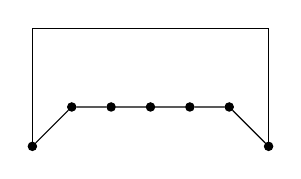
\begin{tikzpicture}[every node/.style={draw,shape=circle,fill=black,inner sep=0pt,minimum size=3pt}]
  \path (0,0) node (p0) {} (.5,.5) node (p1) {} (1,.5) node (p2) {}
  (1.5,.5) node (p3) {} (2,.5) node (p4) {} (2.5,.5) node (p5) {} (3,0) node (p6) { };
  \draw (p0) -- (p1) -- (p2) -- (p3) -- (p4) -- (p5) -- (p6);
  \draw (0,0) -- (0,1.5) -- (3,1.5) -- (3,0);
  \end{tikzpicture}
  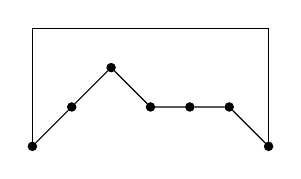
\begin{tikzpicture}[every node/.style={draw,shape=circle,fill=black,inner sep=0pt,minimum size=3pt}]
  \path (0,0) node (p0) {} (.5,.5) node (p1) {} (1,1) node (p2) {}
  (1.5,.5) node (p3) {} (2,.5) node (p4) {} (2.5,.5) node (p5) {} (3,0) node (p6) { };
  \draw (p0) -- (p1) -- (p2) -- (p3) -- (p4) -- (p5) -- (p6);
  \draw (0,0) -- (0,1.5) -- (3,1.5) -- (3,0);
  \end{tikzpicture}
  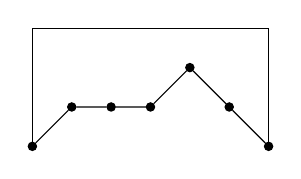
\begin{tikzpicture}[every node/.style={draw,shape=circle,fill=black,inner sep=0pt,minimum size=3pt}]
  \path (0,0) node (p0) {} (.5,.5) node (p1) {} (1,.5) node (p2) {}
  (1.5,.5) node (p3) {} (2,1) node (p4) {} (2.5,.5) node (p5) {} (3,0) node (p6) { };
  \draw (p0) -- (p1) -- (p2) -- (p3) -- (p4) -- (p5) -- (p6);
  \draw (0,0) -- (0,1.5) -- (3,1.5) -- (3,0);
  \end{tikzpicture}

  \#1,2,3,4,5,6,6,8,9,12,14$\to$11 out of 22 have horizontal steps on $x$-axis
\end{enumerate}
\end{document}
